\documentclass{cescg}[2005/11/12]
\usepackage[utf8]{inputenc}


\usepackage{graphicx}  
\usepackage[small,it,labelfont=bf, width=0.9\linewidth]{caption}
\usepackage{times}  % use the Times font

% Title Page
\title{Rapid Modeling of Geology}
\author{Morten Bendiksen}


\begin{document}
\maketitle

\begin{abstract}
Drawing three dimensional models of geological phenomena is today a process requiring training in specific programs that can be very time consuming. For illustration and communication of geological concepts, geologists therefore often limit themselves to drawing on paper or to two dimensional drawing applications.

I propose an approach for making rapid geologic illustrations in 3D. The novel idea for the approach consists of sketch based input on a cube in order to create a layered geological structure. Further details can be added to the layers by sketching geological concepts such as rivers, mountains and valleys. Sedimentary deposits can be created through a procedural modeling approach that employs a volume preserving diffusion algorithm to simulate the flow of depositional material on top of the terrain. Awareness of the geologic domain enables a sparse amount of input strokes to be interpreted into geological structures.

Results show that the proposed approach can be used with success to model geological layers. Compared with a 2D sketch, the creation of a 3D geometry on a computer gives advantages such as perspective control, ease of making changes to the model, etc. The approach shows great promise and can be useful in many situations. A program based on the proposed approach could become a standard way for geologists to draw their illustrations.
\end{abstract}

\section{Introduction}

\begin{figure}[b]
 \centering
 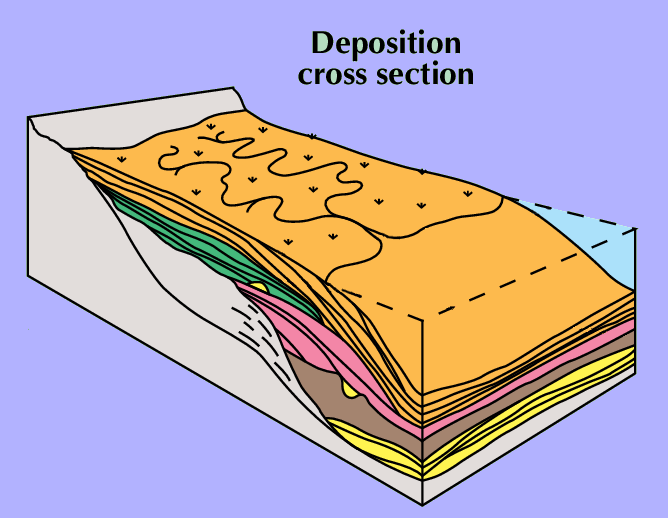
\includegraphics[width=0.7\linewidth]{strataSketch.png}
 % TODO insert reference
 \caption{A typical sketch from a earth science paper. }
 \label{fig:strataSketch}
\end{figure}
It is a common practice to make sketched geological models by hand on either paper or computer. These sketches are used in both professional and educational settings, and facilitate communication and understanding. Geologic phenomena are four dimensional in nature since they occur over time in the three spatial dimensions. There are many techniques and standards for illustrating these phenomena in a two dimensional drawing. One can for example sketch three dimensional phenomena by using perspective drawing techniques, but the model is still confined to the 2D nature of the medium. These techniques and standards can also be limiting  as they require significant time and training to master and understand. Before I started working on this project a problem was identified; there did not exist any tools aimed at helping geologists sketch 3D models for illustration purposes. On the computer it is already possible to make 3D models in traditional modeling approaches. However, existing tools are often complex, aimed 
at creating advanced and detailed models, and usually requires training to understand and use. It is from this background that the goal of this project was formed. 



The goal of this project is to enable the rapid creation of 3D models of geologic structures by creating an approach that lets geologists quickly specify input in an intuitive way that is easy to learn. The model will be used for illustrative purposes to facilitate communication between geologists by letting them create sketched models quicker, help lecturers explain concepts to students by creating models that can be changed interactively, and reduce the need for artistic skills and long training for students to master illustration techniques. The study of sedimentary layer structures and the processes that deform such layers are perhaps the fields of study that has resulted in the most knowledge about the history of the Earth. I concentrate most effort around the creation of rapid modeling techniques for geological layer structures. The aim is to create an approach for the creation of such structures.

\section{Approach}

\begin{figure}
 \centering
 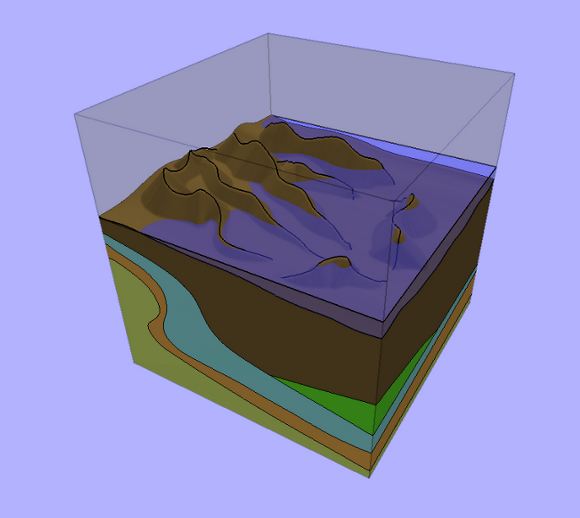
\includegraphics[width=0.7\linewidth]{approachSketch.png}
 % TODO insert reference
 \caption{A typical sketch made with the proposed approach. }
 \label{fig:approachSketch}
\end{figure}

I employ a sketch-based input that is projected onto a transparent cube. Layered geological structures are often sketched in a cube, and I therefore propose to mimic this technique for the sketching interface. The user can rotate around the cube and sketch on the four vertical faces of the cube. On the faces the user sketches the outlines of a surface that will be the top boundary of one of the layer volumes. The surface is then interpolated between the sketched outline. In geology, a surface the is called a horizon. The horizon is also what separates two layers stacked on top of each other. I therefore use the top horizons of previously drawn layers as the bottom boundary of new layers. The user can thus create a stack of layers by adding the layers from bottom to top.

In order to change and model details on the layers, I propose methods for drawing further structure features such as mountains, rivers, valleys and deposits. The user can create ridges, rivers and valleys by sketching on the layers. Separate algorithms for each of the features will then modify the layer surface on which it was drawn. The features the user sketches are positioned on the 2D manifold of the surface it was sketched on, such that a change in the underlying layers representation can be made without having to redraw or manually reposition all the features that exist on that layer. Deposits are created by a procedure that distributes material from the point where the river meets the sea. The material is distributed by a volume preserving diffusion algorithm that considers the topology of the underlying layer surface to create a plausible flow of material from the river.



\end{document}          
